\chapter{РЕЗУЛЬТАТИ ХІРУРГІЧНОГО ЛІКУВАННЯ ПАЦІЄНТІВ З ГЕПАТОБЛАСТОМОЮ}

\section{Порівняльна характеристика оперативних втручань}
Для порівняльного аналізу виконаних оперативних втручань в основній групі та групі порівняння, використовували дані тривалості оперативного втручання, час теплової та холодової ішемії, крововтрати та об'єм переливання компонентів крові (Таб. \ref{tab:operdani}). Статистична значимість відмінностей інтраопераційних показників групи порівняння і основної групи, обчислена за допомогою непараметричних критеріїв для незалежних вибірок Манна-Уїтні.
Тривалість оперативного втручання в резекційній групі склала 240±185 хв., а в трансплантаційній 890±181 хв., що значуще не відрізнялася (p - 0,26, критерій Манна-Уїтні). Різниця медіани тривалості оперативного втручання, пов'язана з складністю оперативного втручання.

\begin{table}[]
\centering
\caption{Інтраопераційні показники при резекції і трансплантації печінки.}
\label{tab:operdani}
\begin{tabular}{|p{0.2\linewidth}|
                 p{0.2\linewidth}|
                 p{0.2\linewidth}|
                 p{0.2\linewidth}|}
\hline
{\color[HTML]{231F20} \textbf{Показник}} &
  {\color[HTML]{231F20} \textbf{Резекційна група (n=81)}} &
  {\color[HTML]{231F20} \textbf{Транс\-план\-тацій\-на група (n=9)}} &
  {\color[HTML]{231F20} \textbf{P}} \\ \hline
{\color[HTML]{231F20} \textbf{Час орперації (хв.)}}        & {\color[HTML]{231F20} 240±185} & {\color[HTML]{231F20} 890±181} & {\color[HTML]{231F20} 0,65} \\ \hline
{\color[HTML]{231F20} \textbf{Крововтрата ( мл.)}}         & {\color[HTML]{231F20} 205±160} & {\color[HTML]{231F20} 460±183} & {\color[HTML]{231F20} 0,68} \\ \hline
{\color[HTML]{231F20} \textbf{Чес теплової ішемії (хв.)}}  & {\color[HTML]{231F20} 30±15}   & {\color[HTML]{231F20} −}       & {\color[HTML]{231F20} 0,72} \\ \hline
{\color[HTML]{231F20} \textbf{Час холодової ішемії (хв.)}} & {\color[HTML]{231F20} −}       & {\color[HTML]{231F20} 55±15}   & {\color[HTML]{231F20} 0,76} \\ \hline
{\color[HTML]{231F20} \textbf{Кількість релапаротомій}} &
  {\color[HTML]{231F20} 6 (11,5\%)} &
  {\color[HTML]{231F20} 1 (12,5\%)} &
  {\color[HTML]{231F20} 0,93} \\ \hline
{\color[HTML]{231F20} \textbf{Тривалість п/о періоду}}     & {\color[HTML]{231F20} 21±7}    & {\color[HTML]{231F20} 48±17}   & {\color[HTML]{231F20} 0,63} \\ \hline
{\color[HTML]{231F20} \textbf{Морбідність}}                & {\color[HTML]{231F20} 17,30\%} & {\color[HTML]{231F20} 11,10\%} & {\color[HTML]{231F20} 0,91} \\ \hline
{\color[HTML]{231F20} \textbf{Летальність}}                & {\color[HTML]{231F20} 4 (5\%)} & {\color[HTML]{231F20} 0 (0\%)} & {\color[HTML]{231F20} 0,95} \\ \hline
\end{tabular}
\end{table}

При аналізі інтраопераційної крововтрати трансплантаційної групи та резекційної групи, також не виявлено істотної різниці показників. Так крововтрата в трансплантацій групі склала 205±160 мл., а в резекційній групі 460±183 мл.. Порівняльний аналіз не показав значущої різниці в обсязі перелитої еритроцитарної маси в обох групах. Також аналіз не показав значущої різниці в обсязі перелитої свіжозамороженої плазми.
Інтраопераційні показники наведено у таблиці (Таб. \ref{tab:operdani})
Час теплової ішемії в резекційній групі склав 30±15 хв. В свою чергу, час холодової ішемії в трансплантаційній групі склав 55±15 хв.. Такий коротких печіод холодової ішемії пов'язаний із виконням тарнсплантації від живого родинного донора, що дозволяє мінімізувати час хододової ішемії до мінімально можливого. 

\section{Порівняльна оцінка ранніх післяопераційних результатів}

Ранні післяопераційні ускладнення наведено у таблиці (Таб. \ref{tab:uscladn}). 
Післяопераційні ускладнення згідно класифікації Dindo-Clavien по групах наведено у таблиці (Таб. \ref{tab:dindopac}). 


\begin{table}[]
\centering
\caption{Ранні післяопераційні ускладнення.}
\label{tab:uscladn}

\begin{tabular}{{|p{0.2\linewidth}|
                 p{0.2\linewidth}|
                 p{0.2\linewidth}|
                 p{0.2\linewidth}|}}
\hline
{\color[HTML]{231F20} \textbf{Ускладнення}} &
  {\color[HTML]{231F20} \textbf{Резекційна група (n=81)}} &
  {\color[HTML]{231F20} \textbf{Транс\-план\-тацій\-на група (n=9)}} &
  {\color[HTML]{231F20} \textbf{P}} \\ \hline
{\color[HTML]{231F20} \textbf{Гостра перфоративна виражка кишечника}} &
  {\color[HTML]{231F20} \textbf{2 (2,5\%)}} &
  {\color[HTML]{231F20} \textbf{−}} &
  {\color[HTML]{231F20} \textbf{0,64}} \\ \hline
{\color[HTML]{231F20} \textbf{Ексудативний плеврит}}              & {\color[HTML]{231F20} 2 (2,5\%)} & {\color[HTML]{231F20} 1 (11,1\%)} & {\color[HTML]{231F20} 0,62} \\ \hline
{\color[HTML]{231F20} \textbf{Підтікання жовчі}}                  & {\color[HTML]{231F20} 4 (4,9\%)} & {\color[HTML]{231F20} 1 (11,1\%)} & {\color[HTML]{231F20} 0,8}  \\ \hline
{\color[HTML]{231F20} \textbf{Інфекція п/о рани}}                 & {\color[HTML]{231F20} 3 (3,7\%)} & {\color[HTML]{231F20} 1 (11,1\%)} & {\color[HTML]{231F20} 0,64} \\ \hline
{\color[HTML]{231F20} \textbf{Пневмонія}}                         & {\color[HTML]{231F20} 3 (3,7\%)} & {\color[HTML]{231F20} 1 (11,1\%)} & {\color[HTML]{231F20} 0,57} \\ \hline
{\color[HTML]{231F20} \textbf{Сепсис, поліорганна недостатність}} & {\color[HTML]{231F20} 2 (2,5\%)} & {\color[HTML]{231F20} −}          & {\color[HTML]{231F20} 0,57} \\ \hline
{\color[HTML]{231F20} \textbf{Внтурішньо\-очеревна кровотеча}}       & {\color[HTML]{231F20} 2 (2,5\%)} & {\color[HTML]{231F20} −}          & {\color[HTML]{231F20} 0,95} \\ \hline
{\color[HTML]{231F20} \textbf{Шлунково-кишкова кровотеча}}        & {\color[HTML]{231F20} 1 (1,2\%)} & {\color[HTML]{231F20} −}          & {\color[HTML]{231F20} }     \\ \hline
\end{tabular}
\end{table}


\begin{table}[]
\centering
\caption{Післяопераційні ускладнення по класифікації Dindo-Clavien.}
\label{tab:dindopac}

\begin{tabular}{|p{0.2\linewidth}|
                 p{0.2\linewidth}|
                 p{0.2\linewidth}|
                 p{0.2\linewidth}|}
\hline
{\color[HTML]{231F20} \textbf{Cтyпiнь}} &
  {\color[HTML]{231F20} \textbf{Резекційна група (n=81)}} &
  {\color[HTML]{231F20} \textbf{Транс\-план\-тацій\-на група (n=9)}} &
  {\color[HTML]{231F20} \textbf{P}} \\ \hline
{\color[HTML]{231F20} \textbf{I}} &
  {\color[HTML]{231F20} \textbf{4}} &
  {\color[HTML]{231F20} \textbf{1}} &
  {\color[HTML]{231F20} \textbf{0,64}} \\ \hline
{\color[HTML]{231F20} \textbf{II}}   & {\color[HTML]{231F20} 1} & {\color[HTML]{231F20} 1} & {\color[HTML]{231F20} 0,62} \\ \hline
{\color[HTML]{231F20} \textbf{IIIa}} & {\color[HTML]{231F20} 5} & {\color[HTML]{231F20} 1} & {\color[HTML]{231F20} 0,8}  \\ \hline
{\color[HTML]{231F20} \textbf{IIIb}} & {\color[HTML]{231F20} 4} & {\color[HTML]{231F20} 1} & {\color[HTML]{231F20} 0,64} \\ \hline
{\color[HTML]{231F20} \textbf{IVa}}  & {\color[HTML]{231F20} 2} & {\color[HTML]{231F20} −} & {\color[HTML]{231F20} 0,57} \\ \hline
{\color[HTML]{231F20} \textbf{IVb}}  & {\color[HTML]{231F20} 2} & {\color[HTML]{231F20} −} & {\color[HTML]{231F20} 0,57} \\ \hline
{\color[HTML]{231F20} \textbf{V}}    & {\color[HTML]{231F20} 4} & {\color[HTML]{231F20} −} & {\color[HTML]{231F20} 0,95} \\ \hline
\end{tabular}
\end{table}



Як один із показників післяопераційних ускладнень проаналізували кількість післяопераційних релапаротомій. У резекційній групі релапаротомії виконано у 6 пацієнтів, що склало 11,5\%, а у трансплантаційній групі у 1 пацієнта (12,5\%). 
Повтрні операції у резекційній групі було виконано у 2 випадках (2,5\%) гострих перфоративних виразок кишечника, що потребувало релапаротомії і опреативної корекції, в той час як в трансплантаційній групі таке ускладнення не спостерігали. Також у 2 випадках (2,5\%) у резекційній групі пацієнтів виникли внутрішньочеревні кровотечі, а також у одного (1,2\%) - шлунково-кишкова кровотеча. Такі ускладнення у трансплантаційній групі зафіксовано не було. 

Ексудативний плеврит, яки потребував пункції або дренування плевральної порожнини, спостерігали у обох групах пацієнтів: у 2 (2,5\%) у резекційній та у одного (1,2\%) в трансплантаційній групі (Таб. \ref{tab:uscladn}). 
У післяопераційному періоді у 3 пацієнтів (3,7\%) у резекційній групі та у одного (1,2\%) в трансплантаційній виникла пневмонія. Сепсис та поліорганну недостатність спостерігали у 2 (2,5\%) пацієнтів. 
Також у 4 (4,9\%) пацієнтів резекційної групи та у 1 (1,2\%) в трансплантаційній виникло підтікання жовчі.

Згідно класифікації післяопераційних ускладнень Dindo-Clavien ускладенння І ступеню зафіксоано у 4 пацієнтів резекційної групи та у 1 трансплантаційної (Таб. \ref{tab:dindopac}). Ускладнення ІІ ступеню, тобто ускладнення, для лікування яких достатньо використання фармакологічних засобів, були зафіксовані по 1 в кожній із груп. Ускладнення ІІІа ступеню по Dindo-Clavien, тобто, ускладення, яке потребує малоінвазивної корекції під місцевою анестезією, виникло у 5 пацієнтів резекційної групи, та у одного трансплантаційної. Ускладнення ступеню ІІІb, тобто ті, що потребували малоінвазивної корекції під загальним знеболенням, були зафіксовані у 4 пацєінтів резекційної групи та у 1 пацієнта трансплантаційної групи. 
По два ускладнення стпеню IVa та IVb по класифікації післяопераційних ускладнень Dindo-Clavien, тобто недостатність одного та декількох органів, що потребує інтенсивної терапії, були зафікосовані у резекційній групі. Таких ускладень у групі пацієнтів, що перенесли трансплантацію частини печінки від живого родинного донора з приводу неоперабельної гепатобластоми печінки, зафікосовано не було (Таб. \ref{tab:dindopac}). Крім того, ускладнення V стпеню, тобто смерть пацієнта, зафіксовано у 4 випдаках у резеційній групі, та не було у трансплантаційній групі.


\section{Порівняльна характеристика морфологічних типів  у пацієнтів з гепатобластомою}

\begin{table}[]
\centering
\caption{Відповідь пухлини на неоадювантну хіміотерапію в залежності від  гістологічного типу гепатобластоми.}
\label{tab:patchim}
\resizebox{\textwidth}{!}{%
\begin{tabular}{|
>{\columncolor[HTML]{FFFFFF}}l |
>{\columncolor[HTML]{FFFFFF}}l |
>{\columncolor[HTML]{FFFFFF}}l |
>{\columncolor[HTML]{FFFFFF}}l |}
\hline
{\color[HTML]{231F20} \textbf{Тип}} &
  {\color[HTML]{231F20} \textbf{Підтип}} &
  {\color[HTML]{231F20} \textbf{Частота повної або часткової відповіді за RECIST}} &
  {\color[HTML]{231F20} \textbf{Значимість відмінностей, p}} \\ \hline
\cellcolor[HTML]{FFFFFF}{\color[HTML]{231F20} } &
  {\color[HTML]{231F20} \textbf{Фетальний підтип}} &
  {\color[HTML]{231F20} \textbf{26 (96,3\%)}} &
  {\color[HTML]{231F20} \textbf{0,03}} \\ \cline{2-4} 
\cellcolor[HTML]{FFFFFF}{\color[HTML]{231F20} } &
  {\color[HTML]{231F20} Змішаний ембріональний / фетальний підтип} &
  {\color[HTML]{231F20} 15 (93,7\%)} &
  {\color[HTML]{231F20} \textbf{0,04}} \\ \cline{2-4} 
\cellcolor[HTML]{FFFFFF}{\color[HTML]{231F20} } &
  {\color[HTML]{231F20} Макротрабекулярний підтип} &
  {\color[HTML]{231F20} 2 (50,0\%)} &
  {\color[HTML]{231F20} 0,67} \\ \cline{2-4} 
\multirow{-4}{*}{\cellcolor[HTML]{FFFFFF}{\color[HTML]{231F20} \textbf{Епітеліальний тип}}} &
  {\color[HTML]{231F20} Дрібноклітинний недиференційований підтип} &
  {\color[HTML]{231F20} 1 (33,3\%)} &
  {\color[HTML]{231F20} 0,75} \\ \hline
\cellcolor[HTML]{FFFFFF}{\color[HTML]{231F20} } &
  {\color[HTML]{231F20} Без тератоїдних особливостей} &
  {\color[HTML]{231F20} 18 (94,7\%)} &
  {\color[HTML]{231F20} \textbf{0,03}} \\ \cline{2-4} 
\multirow{-2}{*}{\cellcolor[HTML]{FFFFFF}{\color[HTML]{231F20} \textbf{Змішаний тип (епітеліальний та мезенхімальний)}}} &
  {\color[HTML]{231F20} З тератоїдними особливостями} &
  {\color[HTML]{231F20} 17 (94,4\%)} &
  {\color[HTML]{231F20} \textbf{0,04}} \\ \hline
{\color[HTML]{231F20} \textbf{Гепатобластома без додаткових особливостей (NOS)}} &
  {\color[HTML]{231F20} } &
  {\color[HTML]{231F20} 3 (100\%)} &
  {\color[HTML]{231F20} \textbf{0,02}} \\ \hline
\end{tabular}%
}
\end{table}

Із 90 пацієнтів у 50 (55,5\%) виявлено гепатобластому епітеліального типу, при чому у 27 (30\% фетальний підтип, 16 пацієнтів (17,8\%) ембріональний підтип, у 4 (4,4\%) макротрабекулярний та у 3 (3,3\%) дрібноклітинні недиференційований підтипи. У 37 пацієнтів (41,1\%) - змішану епітеліальну та мезенхімальну, при чому у 19 із них	(21,1\%) підтип без тератоїдних особливостей, та 18	(20,0\%) з тератоїдними  особливостями, Крім того було 3 пацієнти	(3,33\%) з гепатобластомою без додаткових особливостей (NOS). При оцінці відповіді пухлини на неоадювантну хіміотерапію в залежності від гістологічного типу (підтипу) гепатобластом згідно RECIST, було виявлено найгіршу відповідь у пацієнтів з дрібноклітинним недиференційованим підтипом та макротрабекулярним підтипом (Таб.\ref{tab:patchim}).
Рефрактерність до хіміотерапії була вищою у трансплантаційній групі. У трансплантаційній групі у 78\% випадках при патогістологічному аналізі спостерігався змішаний епітеліально-мезенхімальний тип гепатобластоми менш чутливий до хіміотерапії.

\section{Порівняльна характеристика функціонального стану печінки.}
Функція печінкового залишку та трансплантату оцінювалася нами за допомогою вивчення динаміки рівня загального білірубіну, показників коагулограми, загального білка, альбуміну та цитолітичних ферментів у реципієнтів трансплантаційної та резекційної груп у післяопераційному періоді.
Динаміка рівня загального білірубіну в групах представлена на (Рис. \ref{fig:ZB}). Вихідний рівень білірубіну до операції в групах статистично значимо не відрізнявся і склав 313,50 ± 192,53 та 169,33 ± 177,20 у трансплантаційній та резекційній групі відповідно. В обох групах відмічено зниження рівня білірубіну на 1-3 добу, що, ймовірно, пов'язано як з крововтратою та інфузією замісних розчинів з подальшою гемодилюцією так і з функціонуванням трансплантату.

Починаючи з 4 доби рівень білірубіну в групах статистично значно відрізнявся (Рис. \ref{fig:ZB}). У трансплантаційній групі зниження рівня білірубіну тривало 4-11 діб з нормалізацією на 12 добу. У резекційній групі підвищений рівень білірубіну зберігався до 21-22 доби. Значущість відмінностей між групами була виявлена тестом Крускала-Уолліса та підтверджена тестом Манна-Уітні на 4-7 добу (р=0,01), 8-11 добу(р=0,03), 12-15 добу(р=0,001) , 16-18 добу (р = 0,01), 19-21 добу (р = 0,05). Значущість відмінностей між тимчасовими періодами була виявлена за допомогою критерію Фрідмана та підтверджена за допомогою тесту Вілкоксона на 0 (р=0,024), 1-3(р=0,031), 4-7(р=0,05) та 12-15(р = 0,049) добу.

\begin{figure}[h]
\caption{Динаміка загального білірубіну}
\centering
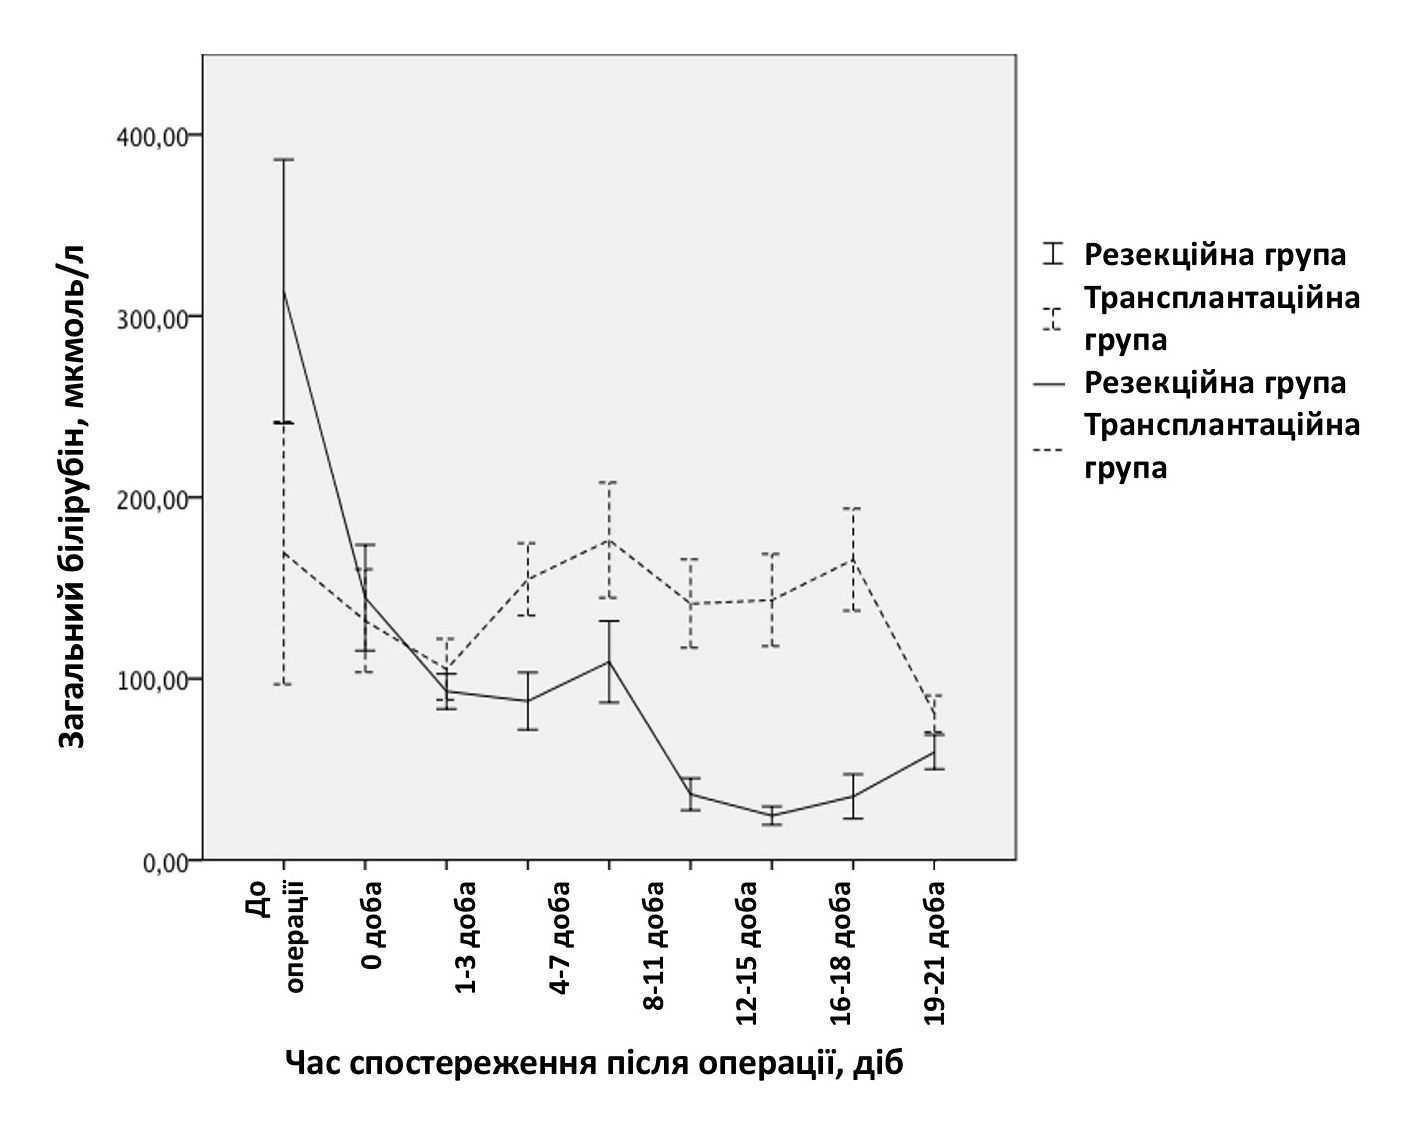
\includegraphics[width=0.7\textwidth]{Illustrations/graf/ZB.jpeg}
\label{fig:ZB} 
\end{figure}

Синтетичну функцію печінки оцінювали за рівнем показників коагулограми, загального білка та альбуміну сироватки крові (Рис. \ref{fig:alb})(Рис. \ref{fig:zbilok})(Рис. \ref{fig:pv}). Протромбіновий час у більшості реципієнтів внаслідок печінкової недостатності був значно підвищений у передопераційному періоді: 29,4±17,2 сек. у загальній вибірці, 31,2±21,0 сек. у трансплантаційній групі та 26±11,2 сек (Рис. \ref{fig:pv}). у резекцийній (відмінність між групами за методом Манна-Уітні статистично не значуща, р = 0,26). На 0-3 добу післяопераційного періоду значення протромбінового часу знижувалося до 257 ± 5 сек. у трансплантаційній групі та 23,5±4,8 у резекційній (р=0,18). Нормалізацію показника відзначали на 4-7 добу в обох групах. Надалі всі пацієнти отримували внутрішньовенну пролонговану інфузію гепарину з розрахунку 2-3 МО на кілограм маси тіла за хвилину для профілактики артеріальних тромбозів. Доза гепарину підбиралася для підтримки протромбінового часу на рівні 20-22 секунд. Після двох тижнів введення гепарину припиняли та призначали таблетовані антиагреганти (дипіридамол). Статистично значимих відмінностей між протромбіновим часом в групах виявлено не було. Значущість відмінностей між тимчасовими періодами була виявлена за допомогою критерію Фрідмана та підтверджена за допомогою тесту Вілкоксона на 1-3 (р=0,042) та 4-7(р=0,034) добу.

\begin{figure}[h]
\caption{Динаміка протромбіновго часу}
\centering
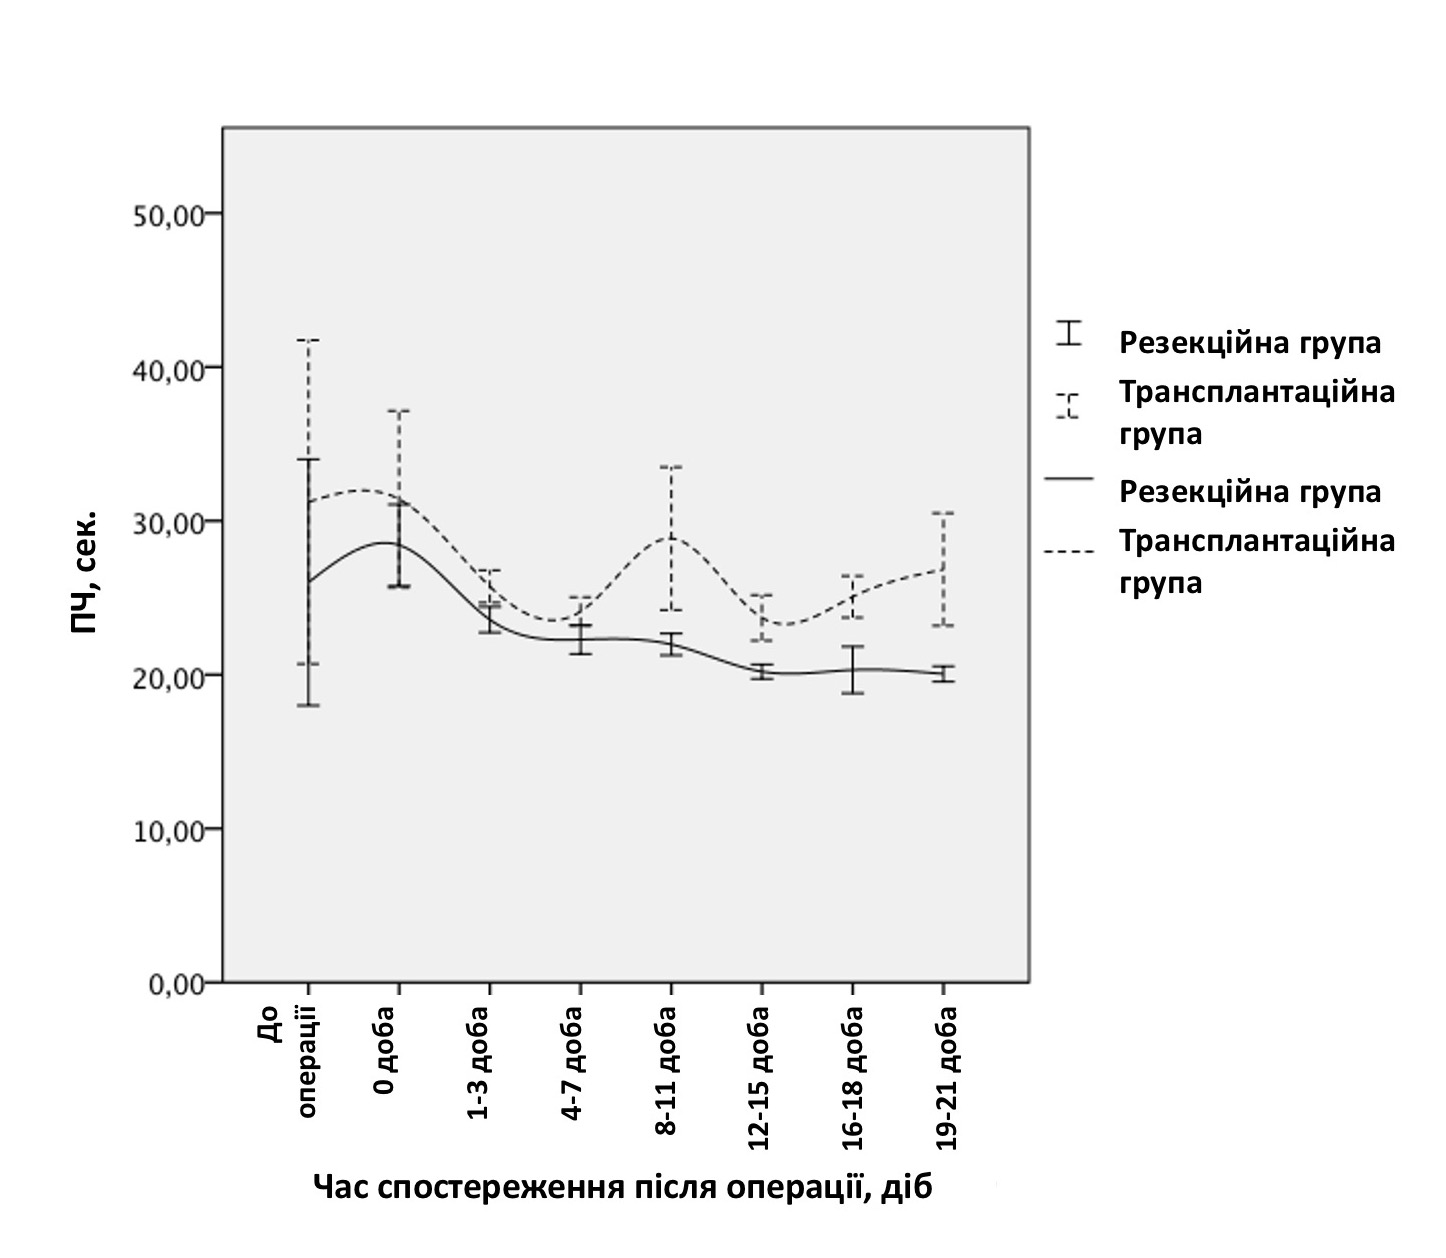
\includegraphics[width=0.7\textwidth]{Illustrations/graf/pv.jpeg}
\label{fig:pv} 
\end{figure}

Концентрація загального білка (Рис. \ref{fig:zbilok}) у сироватці крові реципієнтів резекційної групи та трансплантаційної групи до трансплантації склала 66,2±11,2 г/л та 60,7±6 г/л. На 0-3 добу після операції рівень загального білка в обох групах знижувався до 58,8±5,4 г/л у трансплантаційній та 64,1±5 г/л у резекційній групі. Нормалізація рівня загального білка відзначалася на 4-7 добу до 75±8,1 у трансплантаційній групі та на 12-15 добу до 82±9,2 резекційній. Значущість відмінностей між групами була виявлена тестом Крускала-Уолліса і підтверджена тестом Манна-Уітні до операції (р=0,03), на 0 добу (р=0,043), 1-3 добу (р=0,021), 4-7 добу ( р=0,03), 8-11 добу (р=0,05) та 12-15 добу (р=0,019). Значущість відмінностей між тимчасовими періодами була виявлена за допомогою критерію Фрідмана та підтверджена за допомогою тесту Вілкоксона на 0(р=0,032), 1-3(р=0,045), 4-7(р=0,05) та 12-15(р = 0,015) добу.

\begin{figure}[h]
\caption{Динаміка загального білка}
\centering
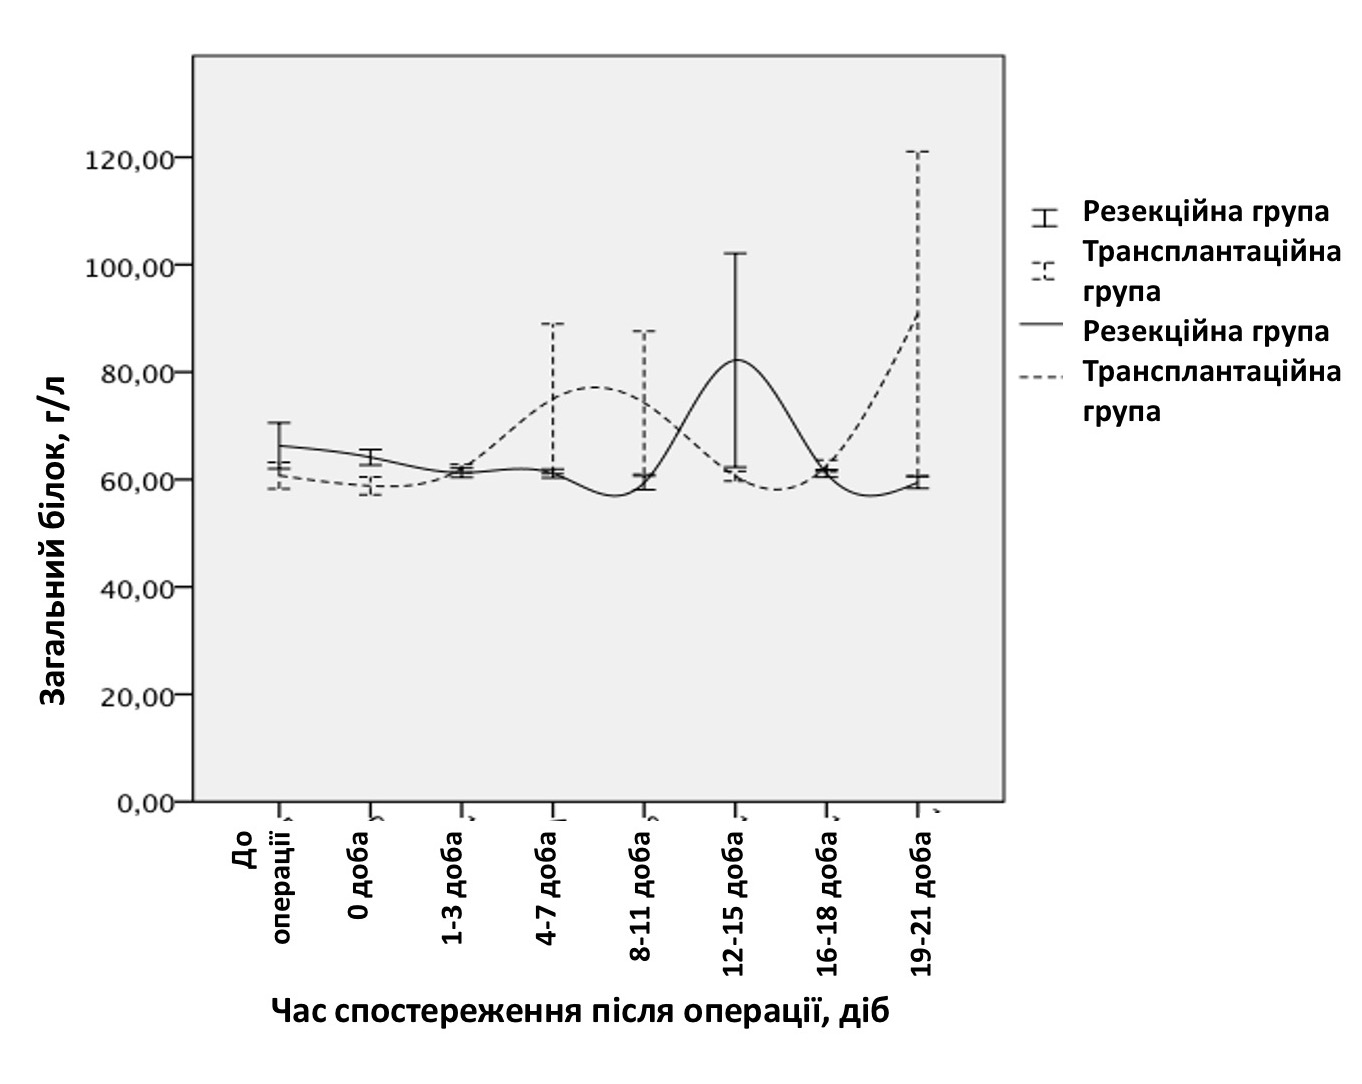
\includegraphics[width=0.7\textwidth]{Illustrations/graf/zbilok.jpeg}
\label{fig:zbilok} 
\end{figure}

Рівень концентрації альбуміну (Рис. \ref{fig:alb}) у сироватці крові обох груп реципієнтів до трансплантації був знижений і значуще між групами не відрізнявся – 32±1,4 г/л у трансплантаційній та 30±2,1 г/л у резекційній групі. У післяопераційному періоді на 0-3 добу в обох групах була відзначена нормалізація рівня білірубіну до 36,6±6 г/л в трансплантаційній та 36,7±5 г/л в резекційній групі внаслідок масивного замісного інтраопераційного переливання альбуміну. Починаючи з 4 доби післяопераційного періоду, рівень альбуміну знижувався в обох групах, але більш значне зниження відзначали резекційній. Різниця між рівнями альбуміну в групах була найбільш виражена на 8-11 добу – 32,8±6 г/л у трансплантаційній та 29,6±3 г/л у резекційній групі.

\begin{figure}[h]
\caption{Динаміка загального альбуміну}
\centering
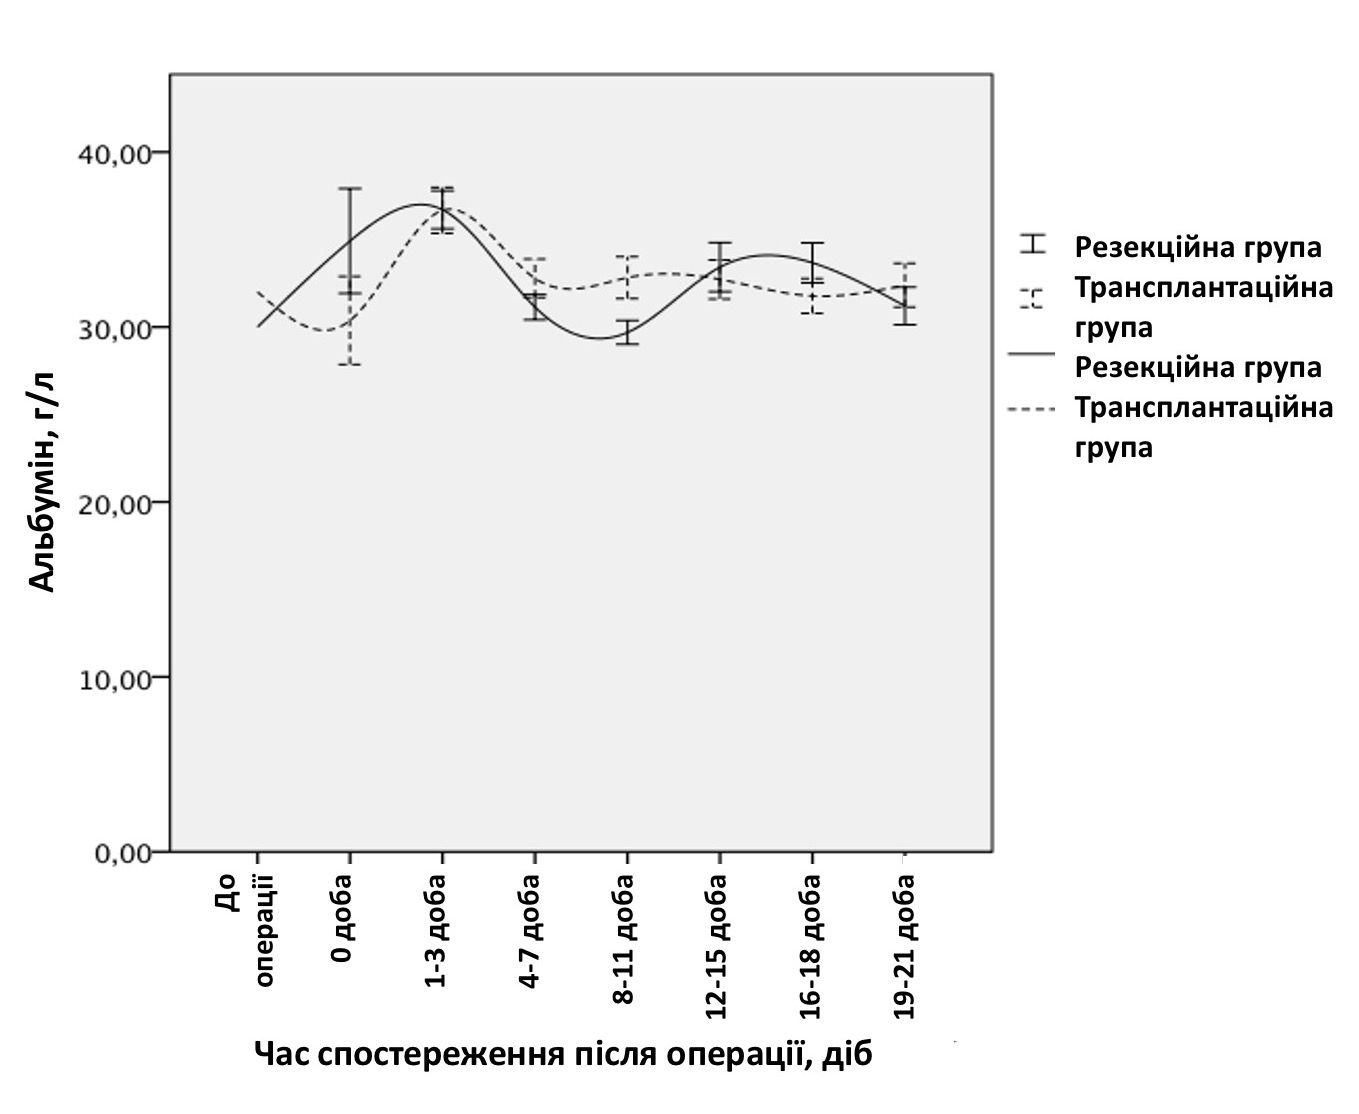
\includegraphics[width=0.7\textwidth]{Illustrations/graf/alb.jpeg}
\label{fig:alb} 
\end{figure}

Починаючи з 12 доби в обох групах відзначали нормалізацію рівня альбуміну – до 33,2±7 г/л у трансплантаційній та 33,4±3 г/л у резекційній групі. Статистична значущість відмінностей між групами була виявлена тестом Крускала-Уолліса та підтверджена тестом Манна-Уітні на 4-7 добу (р=0,021) та 8-11 добу (р=0,01). Значущість відмінностей між тимчасовими періодами була виявлена за допомогою критерію Фрідмана та підтверджена за допомогою тесту Вілкоксона на 0(р=0,024), 1-3(р=0,05), 4-7(р=0,01) та 8-11 (Р = 0,03) добу. Така різниця в динаміці концентрації загального білка та альбуміну сироватки крові обумовлена більшою частотою печінкової недостатності та асцитопродукції у резекційній групі порівняно з трансплантаційною.

Наявність дисциркуляторних змін у паренхімі трансплантату опосередковано оцінювали за рівнем цитолітичних ферментів – аланінамінотрансферази (АЛТ) та аспартатамінотрансферази (АСТ). Рівень АЛТ (Рис. \ref{fig:alt}) в обох групах до операції не відрізнявся, і складав 107±83 ОД у трансплантаційній та 106±97 ОД резекційній групі. У післяопераційному періоді рівень АЛТ зростав в обох групах. Максимальне підвищення активності АЛТ у трансплантаційній групі припадало на 4-7 добу і становило 328±71 ОД, а в резекційній групі на 1-3 добу та становило 272±38 ОД. Нормалізацію активності АЛТ відзначали на 16-18 добу в обох групах. Статистично значущої відмінності між групами не виявлено. Значущість відмінностей між тимчасовими періодами була виявлена за допомогою критерію Фрідмана та підтверджена за допомогою тесту Вілкоксона на 0(р=0,004), 1-3(р=0,041), 4-7(р=0,011) та 8-11(р=0,023) добу.

\begin{figure}[h]
\caption{Динаміка АЛТ}
\centering
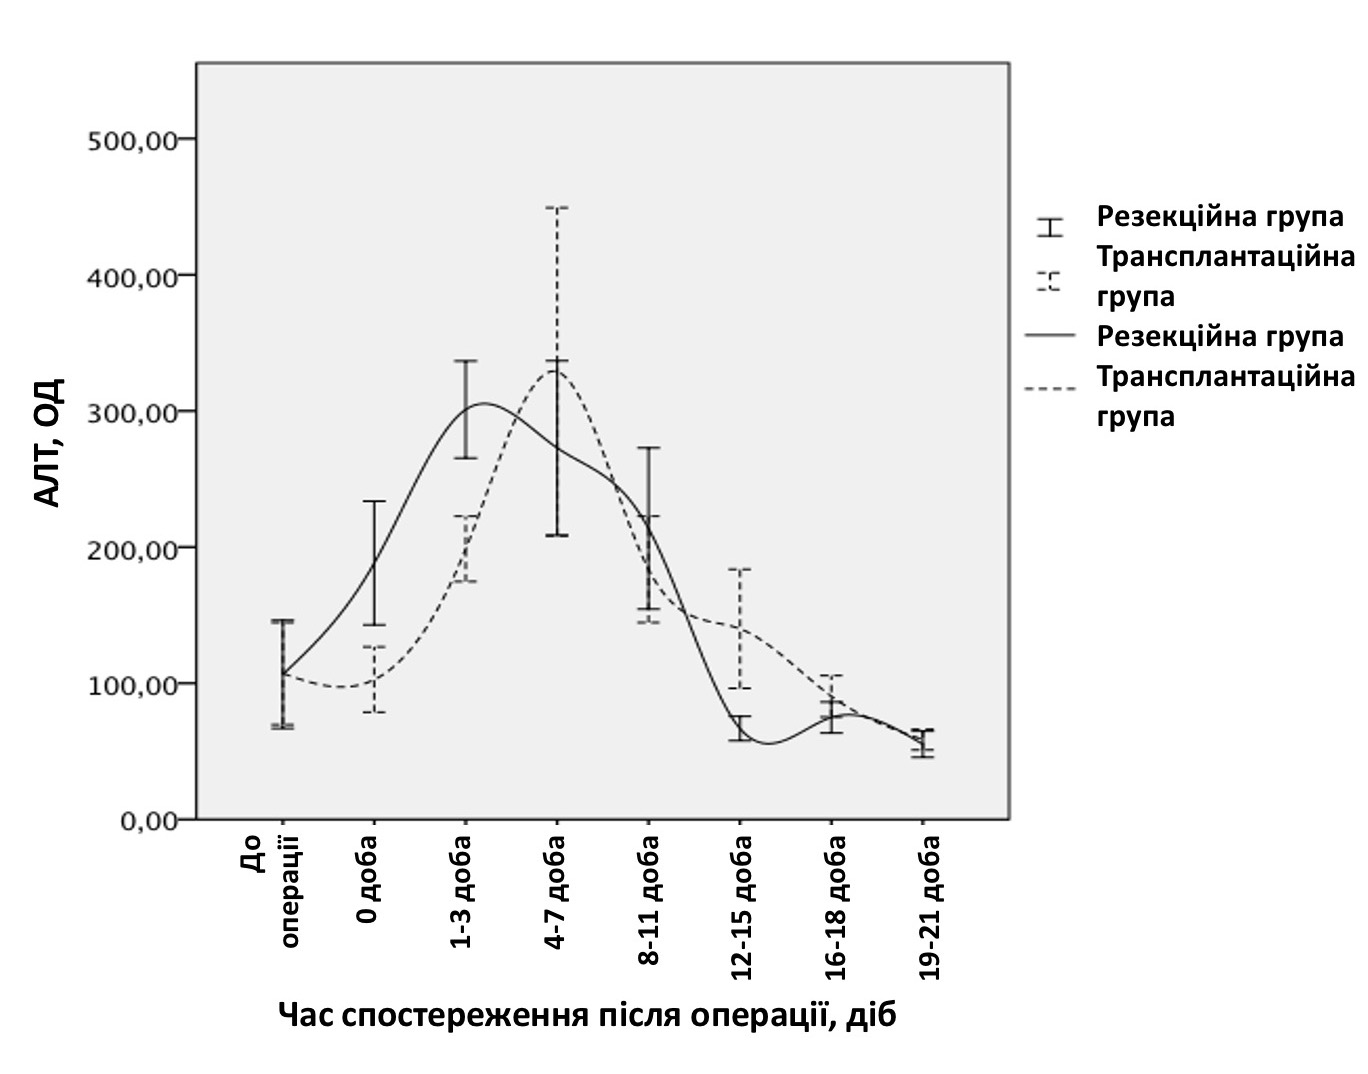
\includegraphics[width=0.7\textwidth]{Illustrations/graf/alt.jpeg}
\label{fig:alt} 
\end{figure}

Рівень АСТ (Рис. \ref{fig:ast}) також у доопераційному періоді у групах статистично значимо не відрізнявся і становив 179±15 ОД у трансплантаційній групі та 177±21 ОД резекційній. У післяопераційному періоді відзначалося підвищення рівня активності АСТ в обох групах. Максимальне підвищення активності АСТ у трансплантаційній групі припадало на 4-7 добу і становило 323 ± 77 ОД, а в резекційній на 1-3 добу і становило 270 ± 18 ОД.

\begin{figure}[h]
\caption{Динаміка АСТ}
\centering
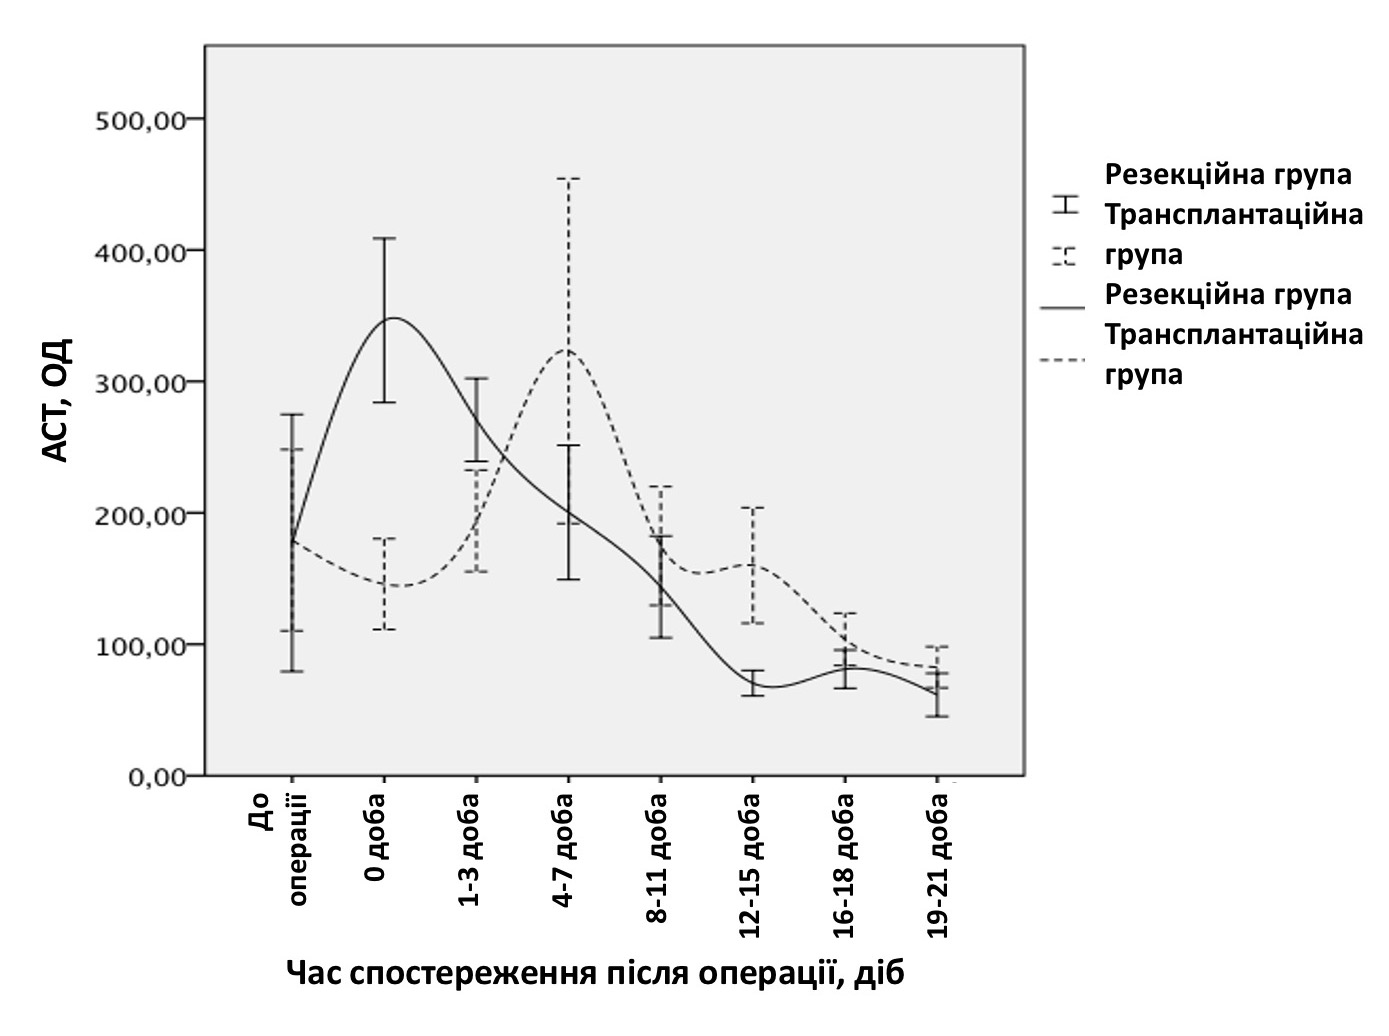
\includegraphics[width=0.7\textwidth]{Illustrations/graf/ast.jpeg}
\label{fig:ast} 
\end{figure}

Нормалізацію активності АЛТ відзначали на 16-18 добу в обох групах. Статистичної значущості відмінностей між групами не виявлено. Значимість відмінностей між тимчасовими періодами була виявлена за допомогою критерію Фрідмана та підтверджена за допомогою тесту Вілкоксона на 0(р=0,03), 1-3(р=0,023), 4-7(р=0,021), 8-11 (p =0,019) та 16-18(р=0,031) добу.
Підвищення активності цитолітичних ферментів у педіатричних реципієнтів пов'язане з наявністю ішемічного ушкодження під час відмивання трансплантату та перфузійного ушкодження при розвитку гіпердинамічного портального кровотоку в ранньому післяопераційному періоді, що підтверджує їх нормалізація на другому тижні післяопераційного періоду.




\section{Порівняльна оцінка віддалених післяопераційних результатів}

Рання післяопераційна летальність в стаціонарі (до 30 діб) в резекційній групі склала 4 (4,9\%) пацієнтів, і не було леталності в трансплантаційній групі. 
Для розрахунку загальної та безрецидивної виживаності по групах використали метод Каплан-Мейєра, значимість відмінностей в групах визначали з допомогою критерія Log-rank и Breslow. криві виживаності представлені на (Рис. \ref{fig:os1}) та (Рис. \ref{fig:dfs1}). Форма кривих свідчить про те, що найбільш критичним печіодом для пацієнтів ж перші 3 місяці післяопераційного періоду. В подальшому післяопераційному періоді ризик летального випадку значно зменшується. 
Для оцінки віддалених результатів хірургічного лікування гепатобластоми з допомогою резекції печінки та трансплантації досліджували виживання протягом 1, 2-х і 3-х років після операції. Загальна 1, 3, 5 річна виживаність у резекційній групі склала 92,3\%, 82,7\%, 71,1\% відповідно. У трансплантаційній групі 1, 3, 5 річна виживаність склала 100\%, 87,5\%, 75\% відповідно (Рис. \ref{fig:os1}).

\begin{figure}[h]
\caption{Загальна виживаність пацієнтів з гепатобластомою.}
\centering
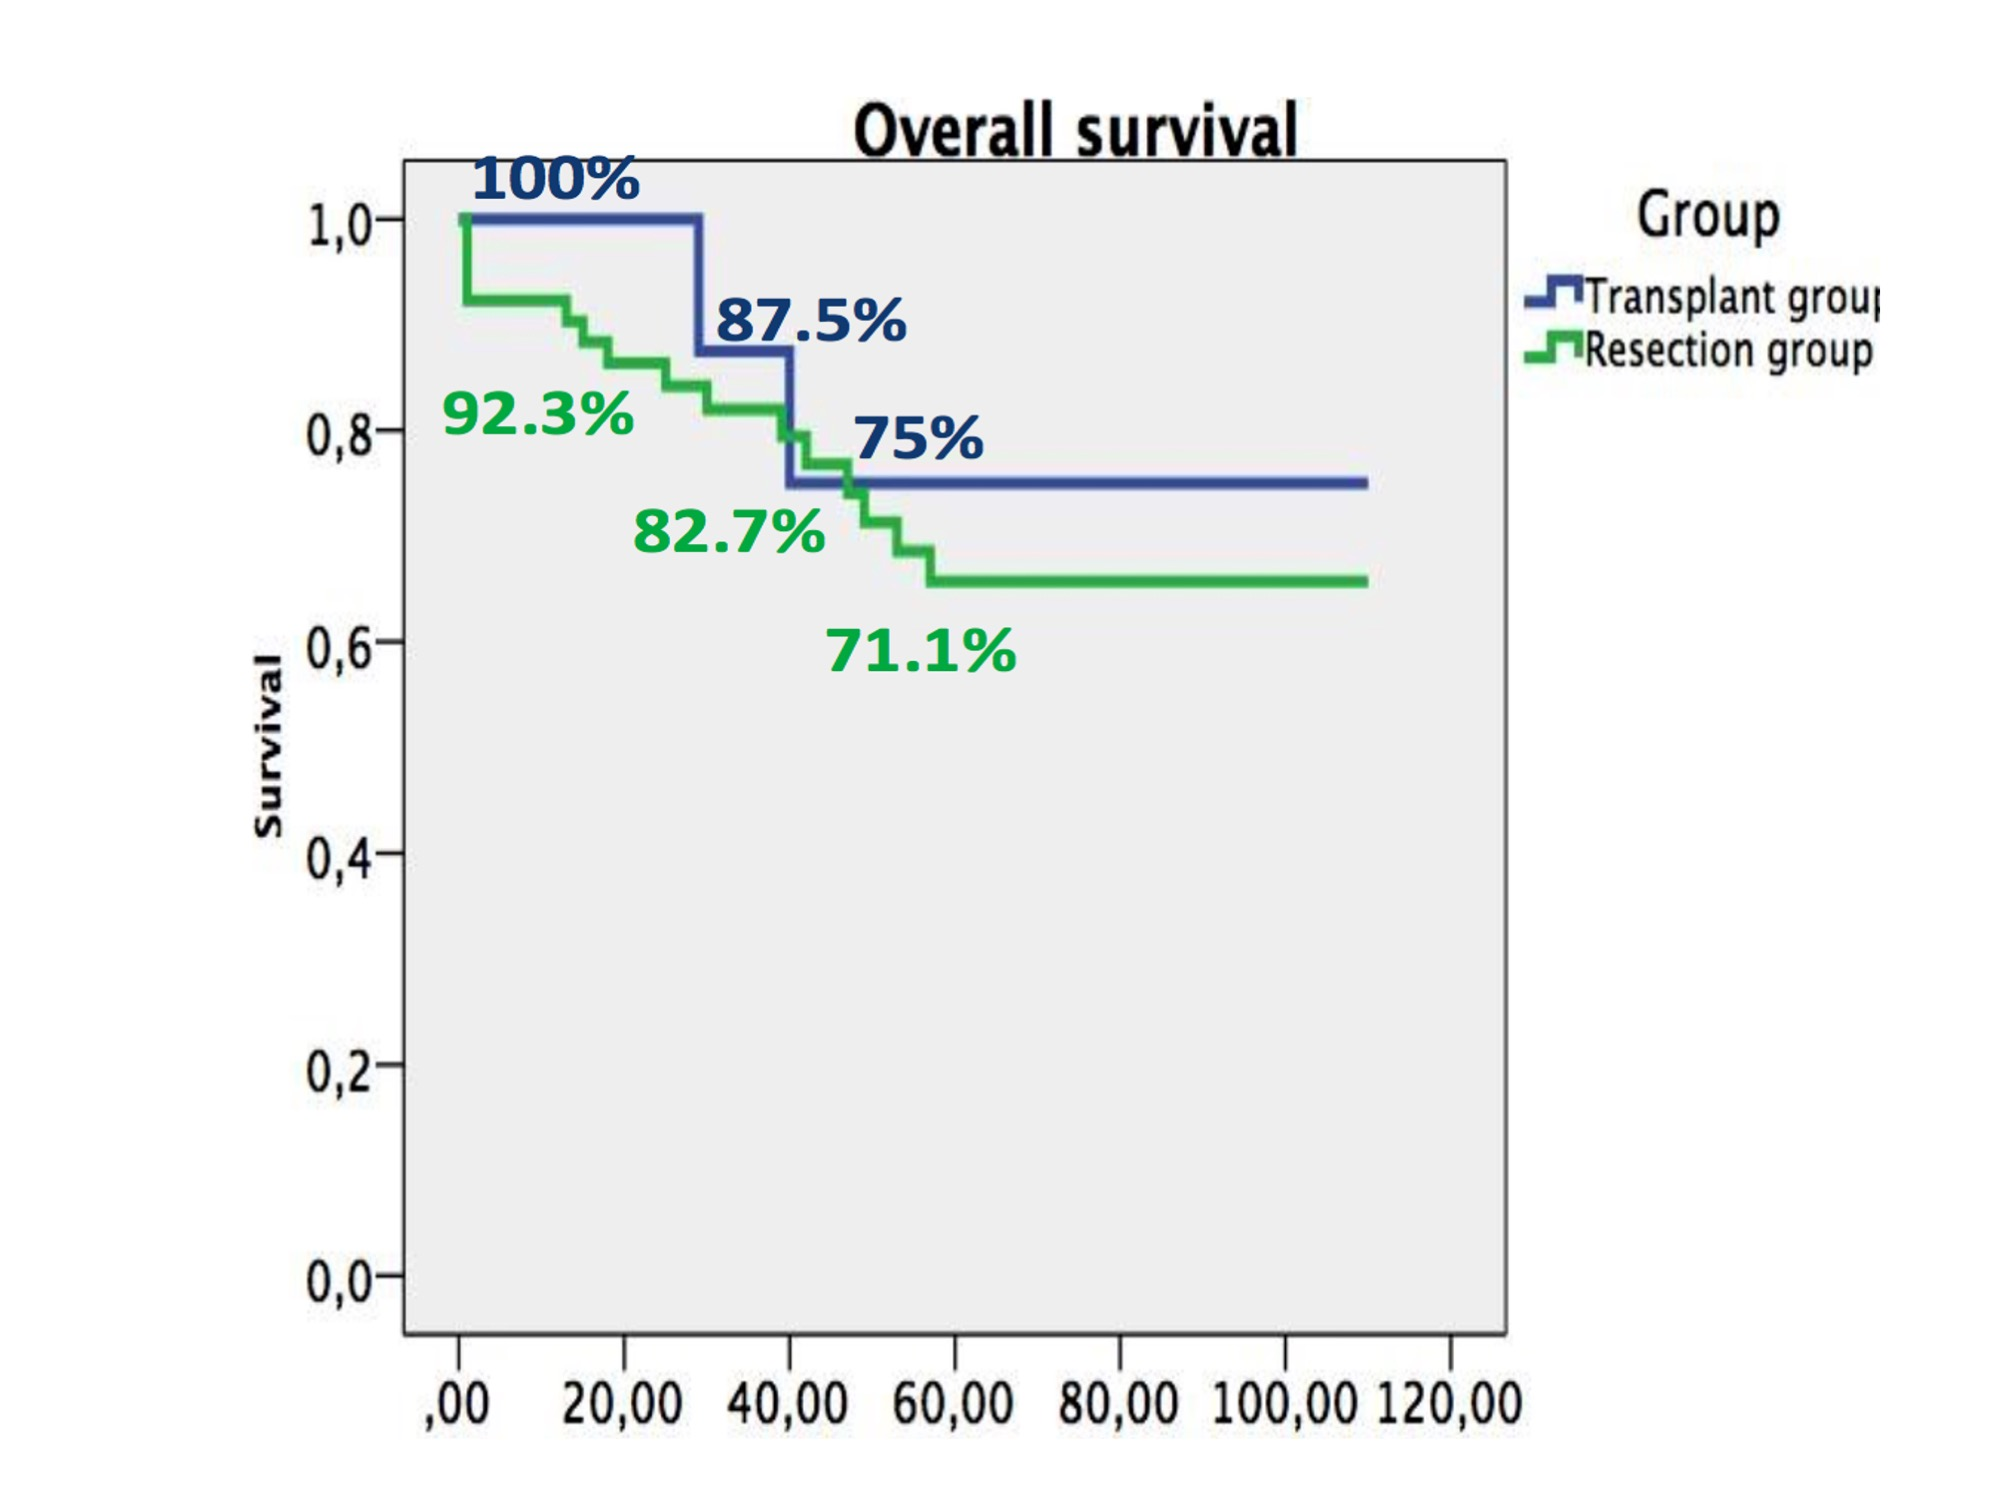
\includegraphics[width=0.8\textwidth]{Illustrations/os1.jpg}
\label{fig:os1} 
\end{figure}


Безрецидивна 1, 3, 5 річна виживаність у резекційній групі склала 86,5\%, 76,6\%, 69,2\% відповідно. У трансплантаційній групі 1, 3, 5 річна виживаність склала 87,5\%, 75,0\%, 62,5\% відповідно (Рис. \ref{fig:dfs1}).

\begin{figure}[h]
\caption{Безрецидивана виживаність пацієнтів з гепатобластомою.}
\centering
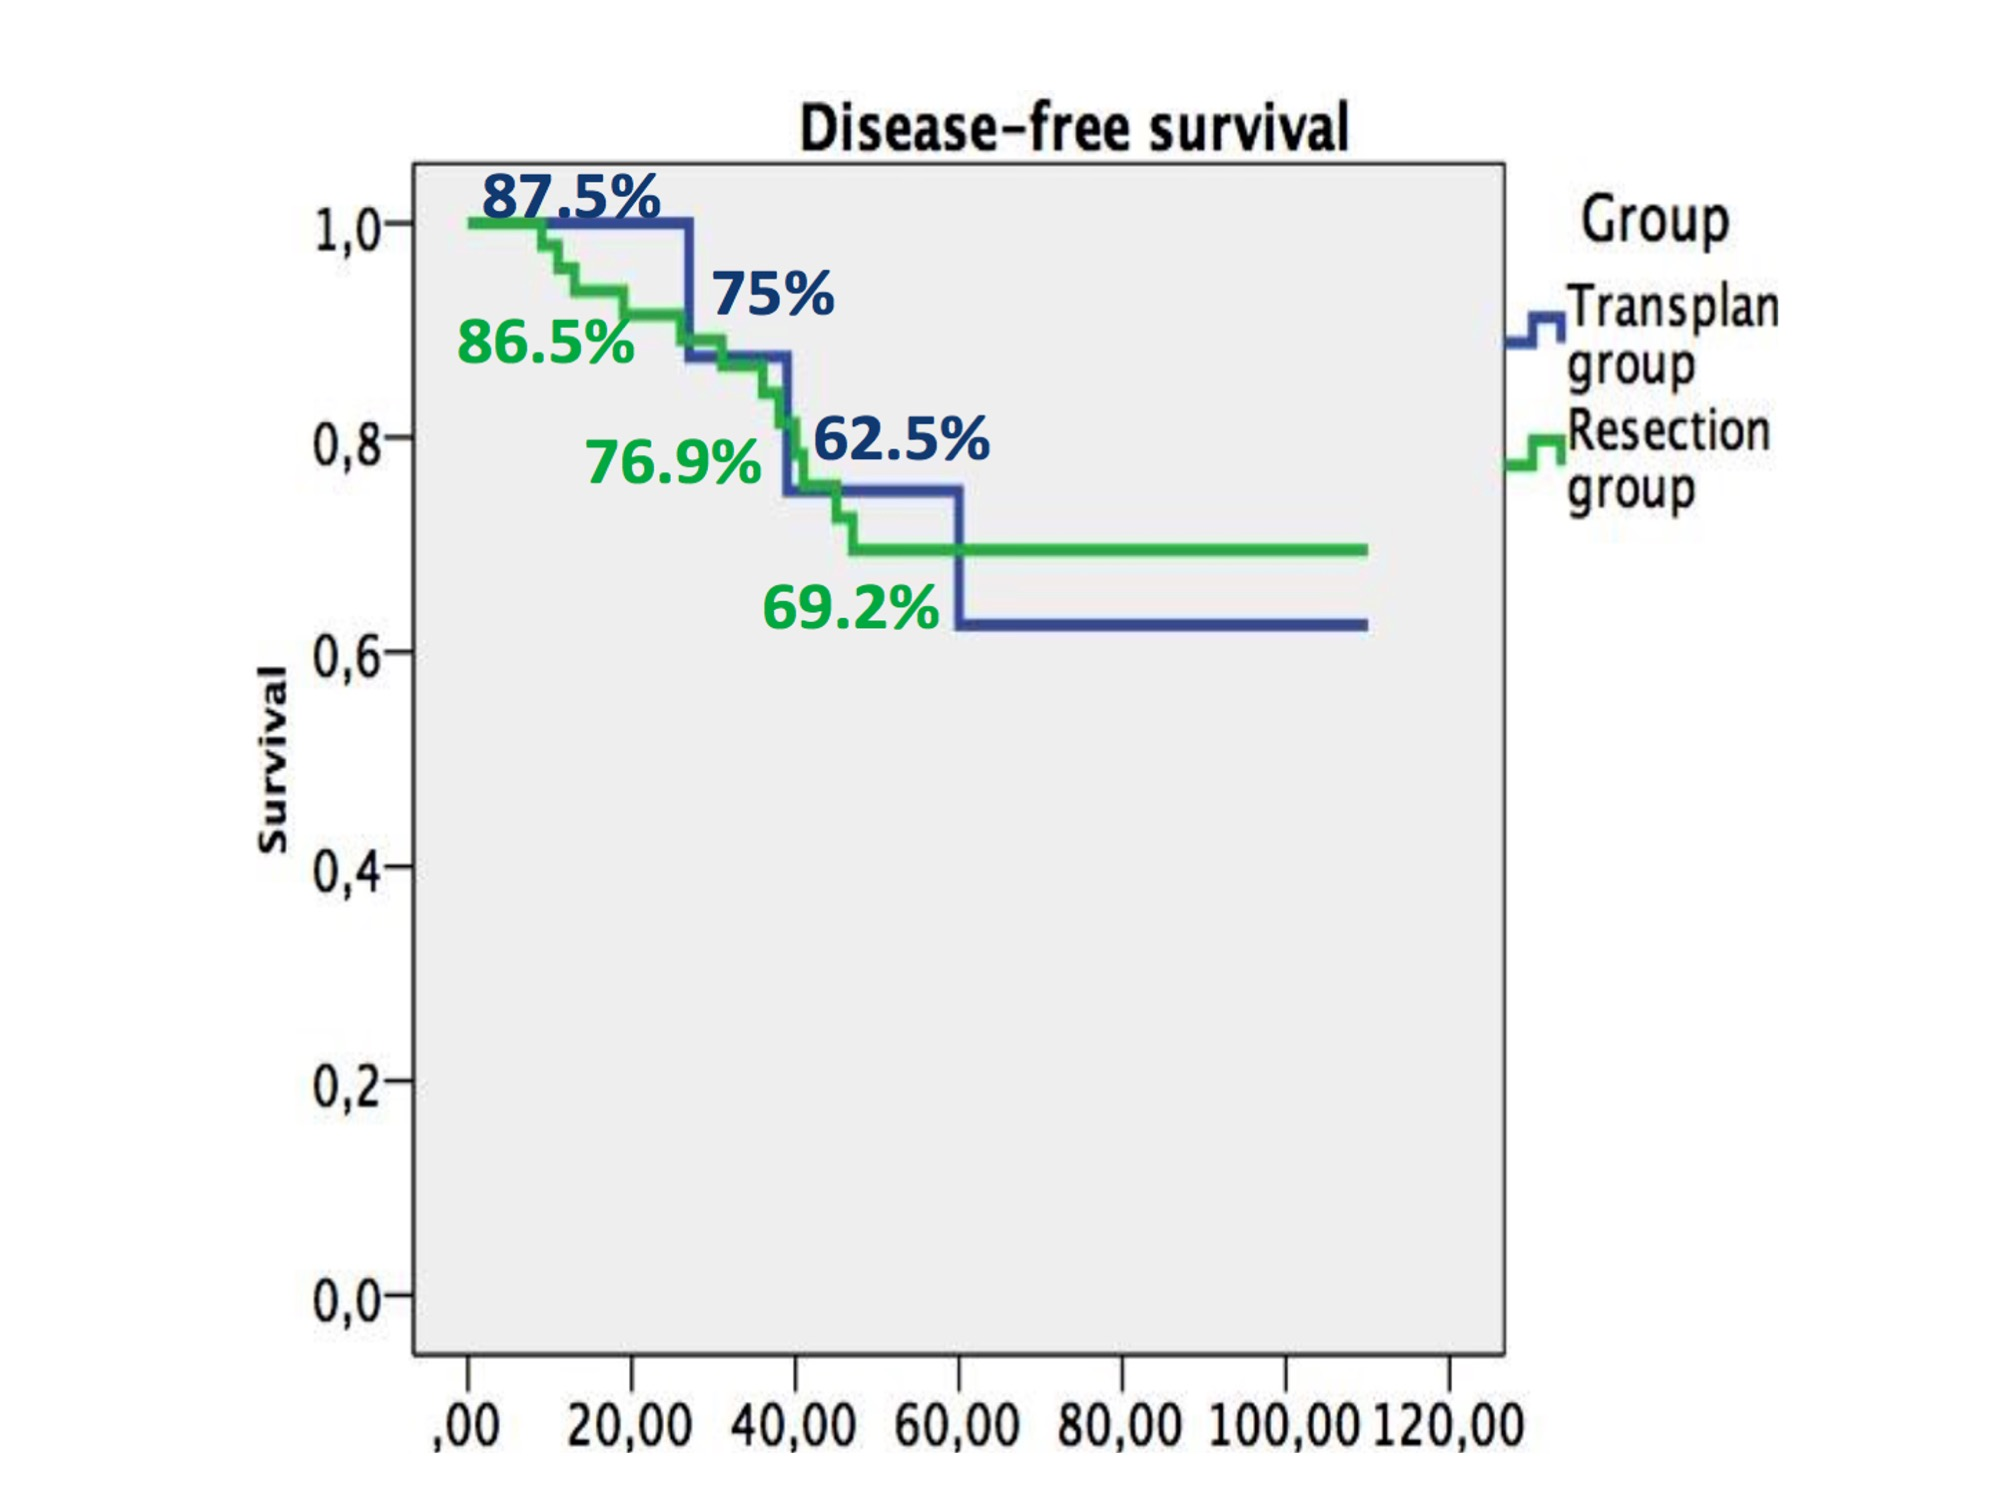
\includegraphics[width=0.8\textwidth]{Illustrations/dfs1.jpg}
\label{fig:dfs1} 
\end{figure}

\section{Алгоритм вибору тактики лікування у пацієнтів з гепатобластомою}
Базуючись на використанні запропонованої нами тактики лікування пацієнтів з гепатобластомою, нами було розроблено алгоритм вибору тактики лiкування у пацiєнтiв з гепатобластомою. Алгоритм базується на результатах доопераційної діагностики та стадіювання пацієнтів Рис. \ref{fig:algoritmmm}).

При визначенні тактики лікування беремо до уваги стадію гепатбластоми по PRETEX, а також її субкласифікації (наявність віддалених метастазів, інвазії в ворітну вену, печінкові або нижню порожнисту вени). 
Після чого визначаємо групу ризику пацієнта по системі CHICS (Children’s Hepatic Tumors International Collaboration`s Stratification), де беремо до уваги такі показники як вік, рівень АФП, інвазію судин та наявність метастазів пухлини та розприділяємо пацієнтів на групи ризику: LR – група низького ризику, IR – група середнього ризику, HR – група високого ризику та VHR – група вкрай високого ризику (Рис. \ref{tab:risk}).

Наступним етапом діагностики є біопсія пухлини. 
В залежності від групи ризику призначається неоадювантна хіміотерапія. 

Після отримання неоадювантної хіміотерапії та нормальлізації гематологічних показників крові, виконується оперативне втручання. Об'єм оперативного втручання залежить від стадії гепатобластоми. За звичай при пухлинах PRETEX І-ІІІ виконували резекції печінки, при PRETEX IV - трансплантацію печінки (Рис. \ref{fig:algoritmmm}).

При наявності резектабельного метастазу, після неоадювантної хіміотерапії при стабілізації пухлини та метастазу проводили метастазектомію. Після оперативного лікування (резекції, тарнсплантації, метастазектомії) після нормалізації стану пацієнта проводили адювантну хіміотерапіз згідно плану (Рис. \ref{fig:algoritmmm}).

В післяопераційному періоді проводимо спостереження у у випадку появи рецидиву або метастазування проводимо повторну резекцію печінки або метастазектомію. 

\begin{figure}[h]
\caption{Алгоритм діагностики і лікування гепатобластоми в залежності від групи ризику}
\centering
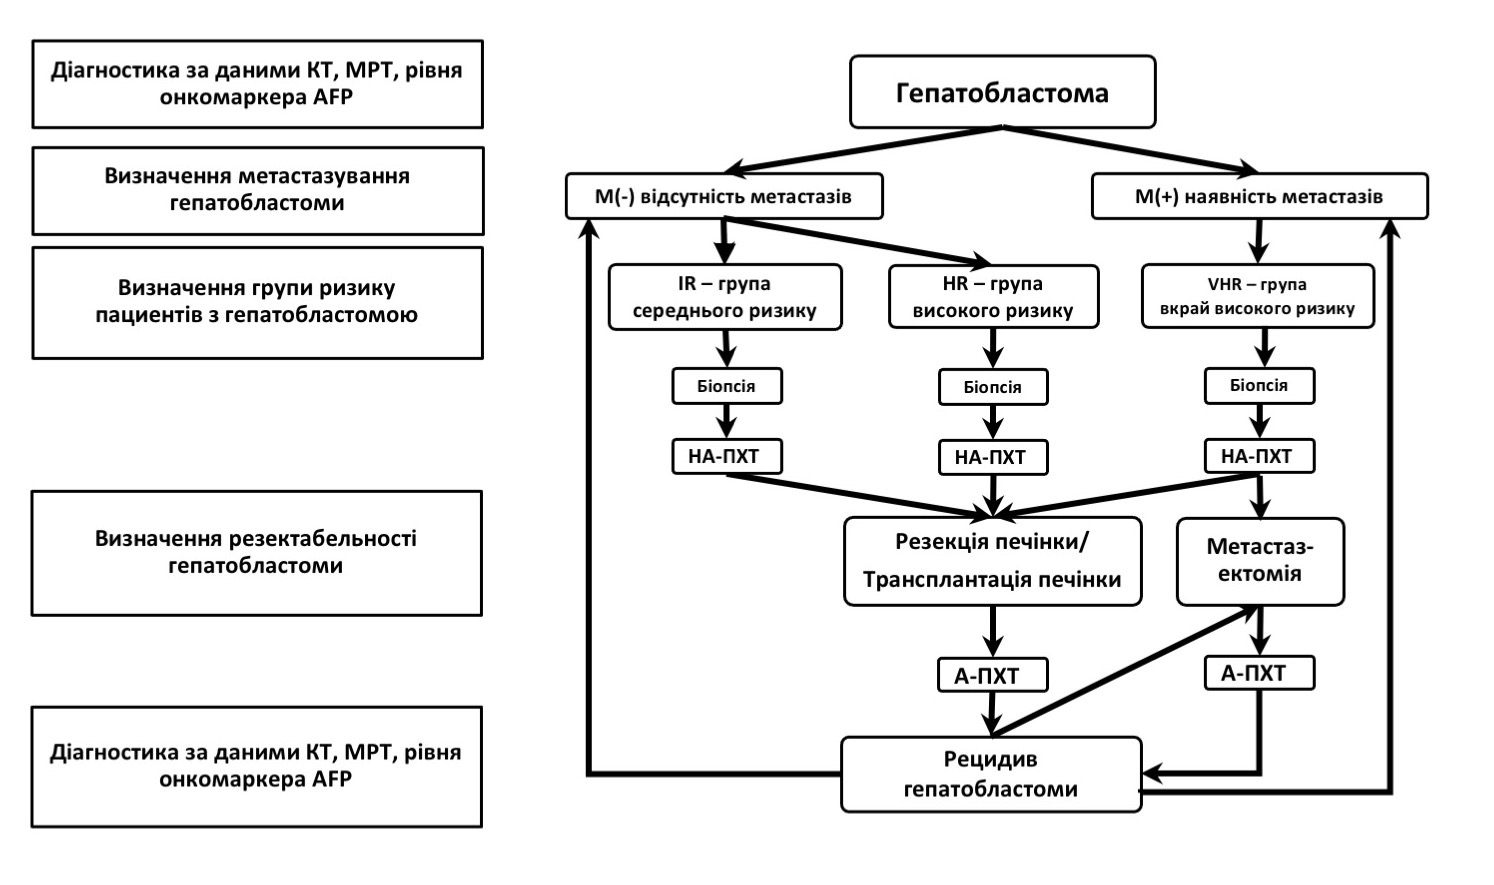
\includegraphics[width=0.9\textwidth]{Illustrations/algoritmmm.jpg}
\label{fig:algoritmmm} 
\end{figure}